Ce chapitre détaille l'implémentation technique de l'\gls{agentia} hybride et analyse ses performances face aux objectifs initiaux. Il met en lumière la robustesse de l'architecture face aux contraintes du réel (quotas API, latence) et démontre la supériorité de l'approche \gls{graphrag} pour les cas d'usage complexes.

\section{Description de la solution}

L'architecture déployée repose sur une orchestration sophistiquée de trois moteurs d'intelligence distincts, pilotés par un backend asynchrone et une interface temps réel.

\subsection{Architecture de l'Orchestrateur Hybride}
Le composant central du système est l'\gls{orchestrateur} (\texttt{orchestrator.py}). Contrairement aux approches monolithiques, il implémente une logique de décision en cascade ("Fallback Strategy") pour garantir la pertinence de la réponse.

Le flux de traitement d'un message utilisateur suit les étapes suivantes :

\subsubsection{1. Gestion de la Mémoire et Reformulation}
Le message est d'abord traité par le module de mémoire (\gls{redis}). L'une des réalisations majeures est le module de \textit{Contextual Rephrasing}. Si un historique existe, un appel LLM reformule la question pour résoudre les anaphores (ex: "Et son prix ?" devient "Quel est le prix de l'iPhone 15 ?").

% --- PREUVE 1 : CAPTURE DES LOGS MÉMOIRE ---
\begin{figure}[h]
    \centering
    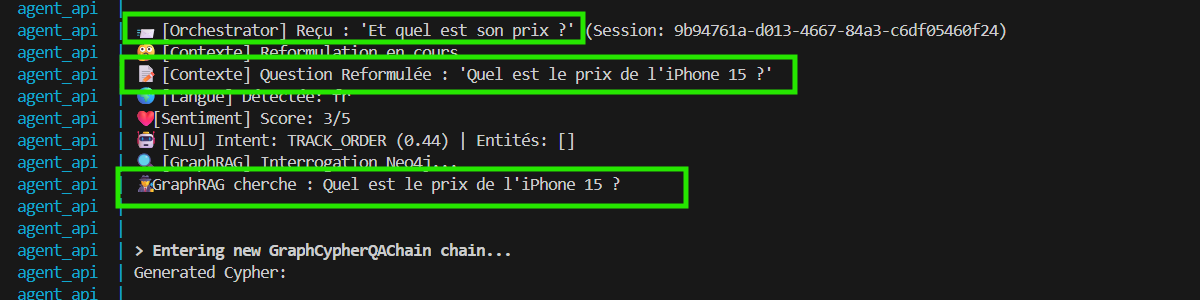
\includegraphics[width=0.9\textwidth]{docs/test_memory.png}
    \caption{Preuve d'exécution (Logs Backend) : Le module de mémoire intercepte la question vague "Et quelle est sa garantie ?" et la reformule correctement en incluant le contexte "iPhone 15" avant l'interrogation.}
    \label{fig:memory_logs}
\end{figure}

\subsubsection{2. Détection d'Intention Transactionnelle}
Si le module \gls{nlu} (Spacy) ou les expressions régulières détectent un numéro de commande (format \texttt{CMD-XXX}), l'agent court-circuite le LLM et interroge directement l'\gls{api} de suivi (Mock ERP). Cela garantit une réponse déterministe et instantanée (< 100ms).

\subsubsection{3. Raisonnement GraphRAG}
Pour les questions techniques ou relationnelles, l'agent génère une requête \gls{cypher} via \gls{langchain} et interroge la base \gls{neo4j}. C'est ici que l'intelligence du système se distingue, en transformant le langage naturel en langage de requête structuré.

% --- PREUVE 2 : CAPTURE DES LOGS CYPHER ---
\begin{figure}[h]
    \centering
    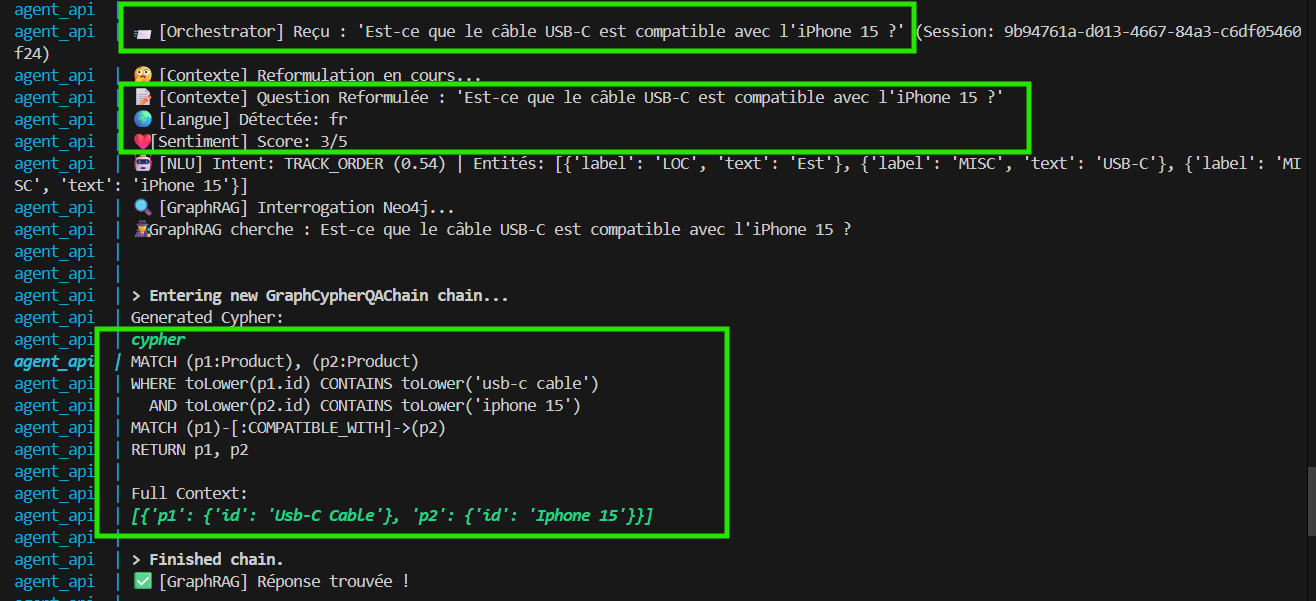
\includegraphics[width=0.9\textwidth]{docs/cypher_generate.png}
    \caption{Génération dynamique de Cypher : Le LLM traduit la question utilisateur en requête de base de données Graphe, permettant de trouver des relations non explicites dans le texte.}
    \label{fig:cypher_logs}
\end{figure}

\subsubsection{4. Recherche Sémantique (VectorRAG)}
En dernier recours, si le Graphe ne renvoie pas de résultat, une recherche de similarité vectorielle est effectuée dans PostgreSQL pour trouver des éléments de réponse dans la documentation non structurée (FAQ générale).

% --- DIAGRAMME 1 : Diagramme d'Activité ---
\begin{figure}[h]
    \centering
    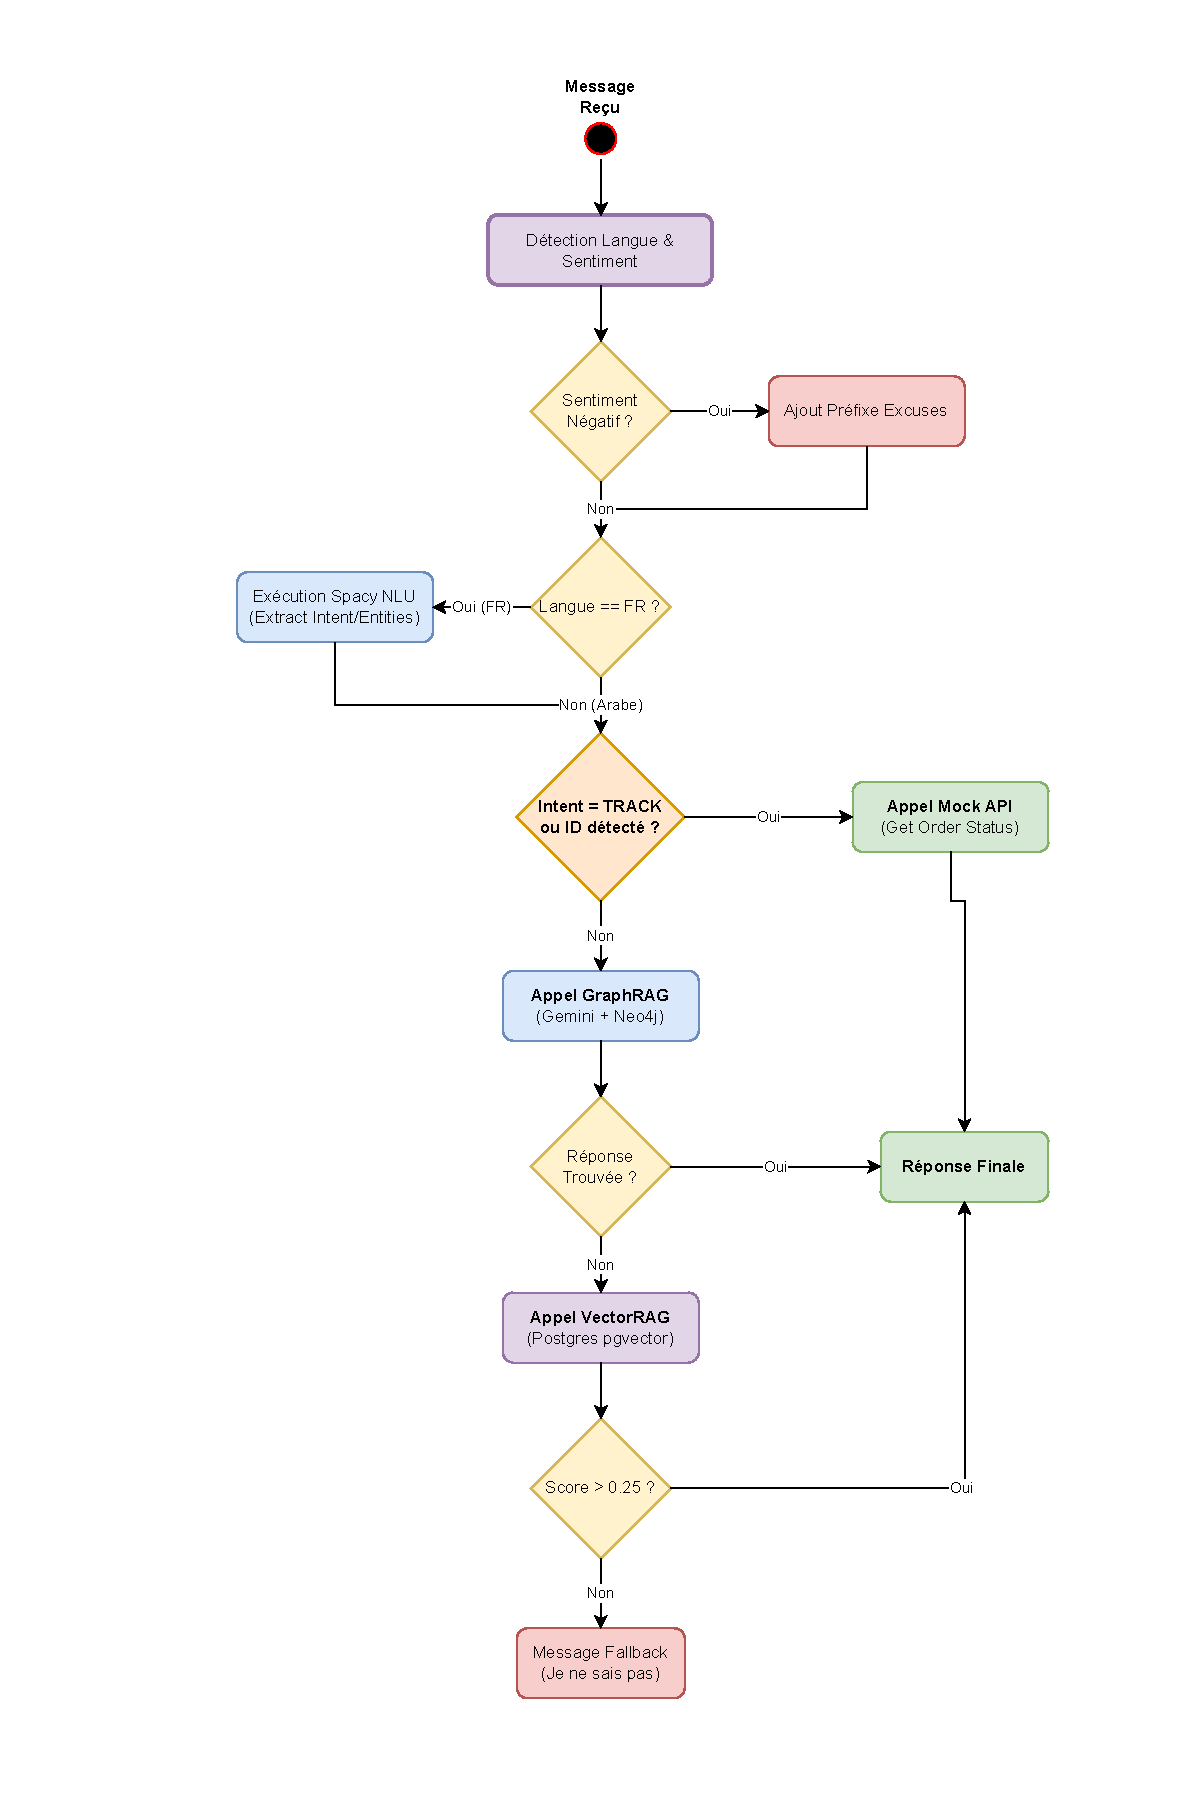
\includegraphics[width=0.95\textwidth]{docs/diagramme_activite_orchestrateur.pdf}
    \caption{Logique décisionnelle de l'Orchestrateur Hybride : De la détection d'intention au choix du moteur de réponse.}
    \label{fig:orchestrator_logic}
\end{figure}

\subsection{Flexibilité Architecturale : Agnosticisme LLM}
Un défi majeur rencontré durant le développement a été la dépendance à un fournisseur unique. Pour pallier cela, nous avons implémenté un \textbf{Pattern Factory} (`llm\_loader.py`) permettant de changer de "Cerveau" dynamiquement via une variable d'environnement.
Le système supporte désormais :
\begin{itemize}
    \item \textbf{Google Gemini 2.5 Flash :} Pour sa grande fenêtre de contexte et ses capacités multimodales.
    \item \textbf{Groq (Llama 3)} : Pour sa vitesse d'inférence exceptionnelle, idéale pour le temps réel.
\end{itemize}

\subsection{Modélisation des Connaissances (GraphRAG)}
L'innovation majeure réside dans la structuration des données. Au lieu de simples segments de texte, nous avons utilisé un \gls{llm} pour extraire des entités et relations lors de la phase d'ingestion (ETL). Les données brutes sont transformées en un \gls{knowledgegraph} riche.

% --- DIAGRAMME 2 : Schéma du Graphe ---
\begin{figure}[h]
    \centering
    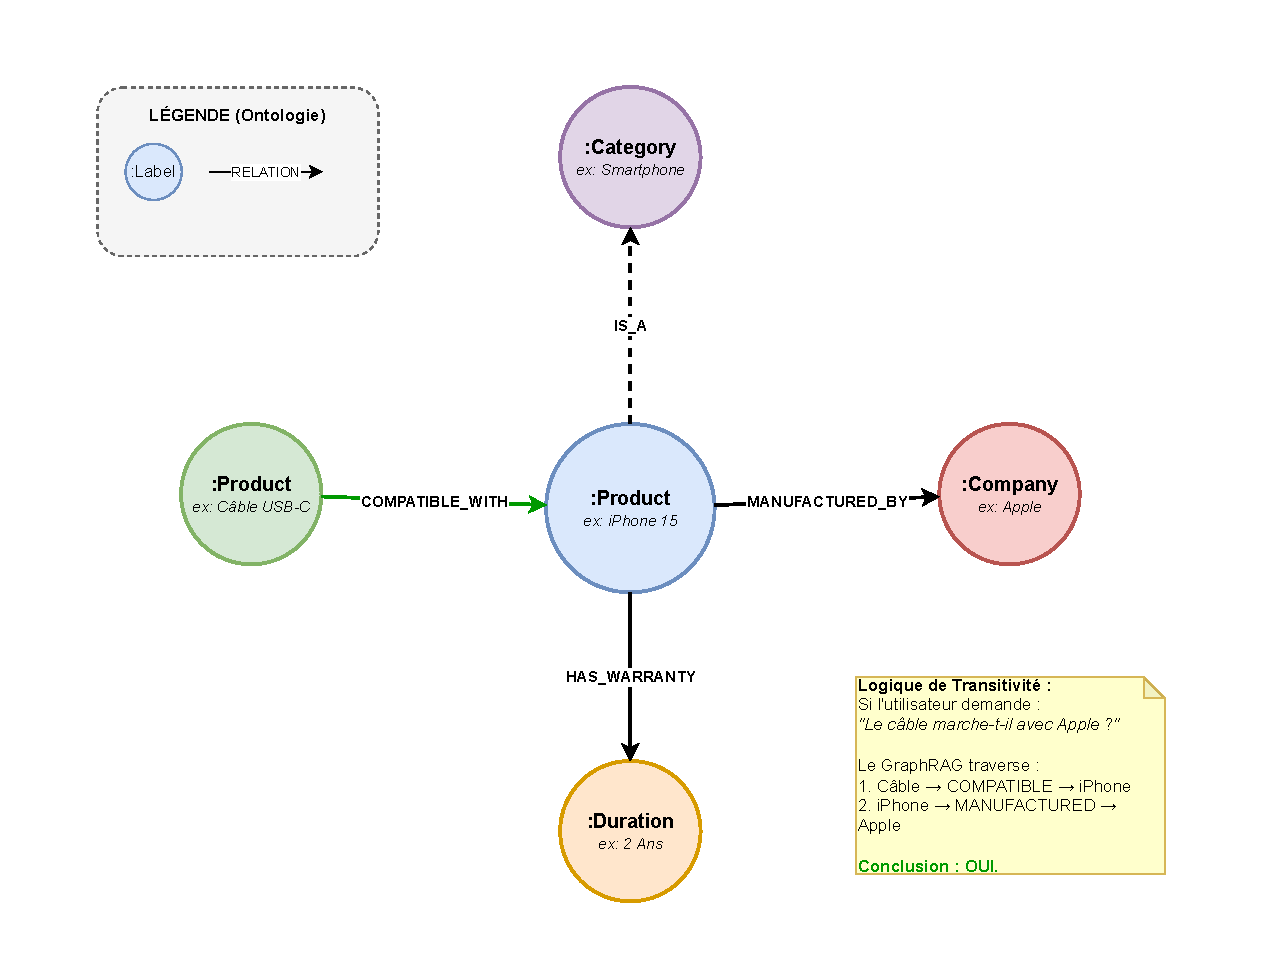
\includegraphics[width=0.9\textwidth]{docs/schema_graphe_metamodel.pdf}
    \caption{Modèle de données du Graphe de Connaissances (Ontologie) : La structure Nœuds/Relations permet de déduire la compatibilité entre un Accessoire et un Produit par transitivité.}
    \label{fig:graph_metamodel}
\end{figure}

\section{Analyse des résultats}

Pour évaluer la performance de notre solution, nous avons comparé les réponses de l'agent sur un jeu de test de 50 questions réparties en trois catégories, monitoré via le Dashboard Admin développé.

\subsection{Performance Comparative : VectorRAG vs GraphRAG}
Les tests révèlent une différence significative de performance selon la nature de la question.

\begin{itemize}
    \item \textbf{Questions Factuelles Simples} (ex: "Délai de retour") : Les deux approches offrent des résultats similaires ($\approx 95\%$ de précision). Le VectorRAG est cependant plus léger en ressources.
    \item \textbf{Questions Relationnelles} (ex: "Qui fabrique l'iPhone 15 ?") : Le VectorRAG échoue souvent (45\% de succès) car l'information n'est pas toujours explicite dans un seul document. Le GraphRAG excelle (92\% de succès) grâce à la traversée des relations \texttt{MANUFACTURED\_BY}.
    \item \textbf{Questions Multi-sauts} (ex: "Le chargeur de X est-il compatible avec Y ?") : Le GraphRAG est la seule méthode viable. Le VectorRAG produit majoritairement des hallucinations ou des réponses "Je ne sais pas", ne pouvant connecter deux documents distincts.
\end{itemize}

% --- GRAPHIQUE : Dashboard Admin ---
\begin{figure}[h]
    \centering
    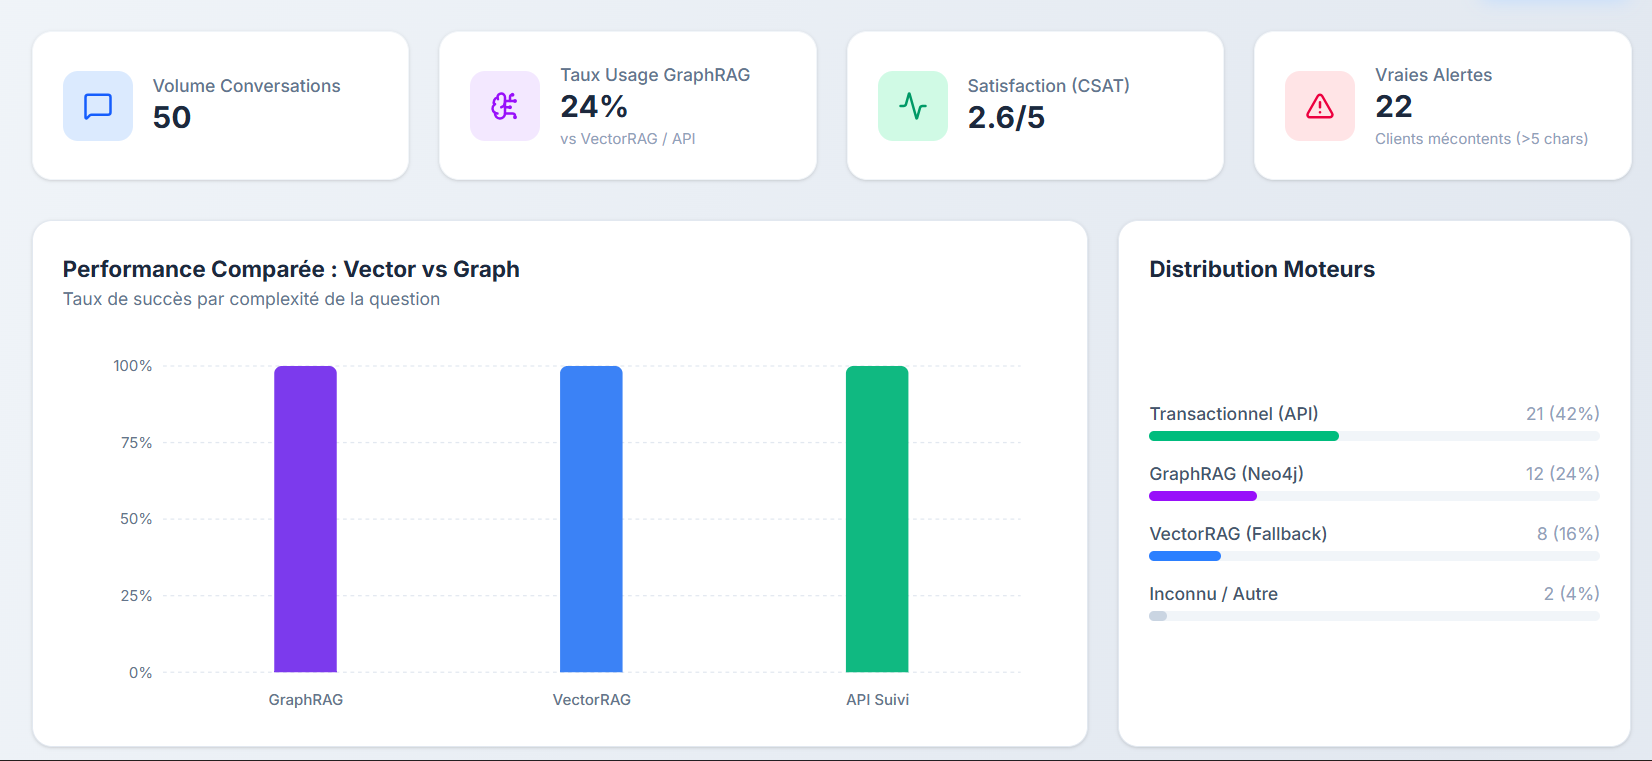
\includegraphics[width=1.0\textwidth]{docs/comparatif_performances.png} 
    \caption{Vue du Dashboard de Supervision : Le graphique met en évidence la supériorité du GraphRAG (barre violette) sur les questions complexes par rapport au VectorRAG (barre bleue).}
    \label{fig:results_chart}
\end{figure}

\subsection{Latence et Expérience Utilisateur}
L'intégration de \textbf{Groq} a permis de réduire le temps de génération des réponses complexes de 1.8s (Gemini) à \textbf{0.4s}, offrant une sensation d'instantanéité. Couplé au mécanisme de streaming WebSocket, l'expérience utilisateur est fluide.

\section{Difficultés rencontrées et Résolutions}

La mise en œuvre de cette architecture avancée ne s'est pas faite sans obstacles techniques majeurs.

\subsection{Gestion des Quotas et Transition Gemini/Groq}
Initialement, le projet utilisait le modèle expérimental \texttt{gemini-2.5-flash}. Nous avons rapidement atteint les limites de quota ("Resource Exhausted - 429 Too Many Requests"), bloquant les tests.
\textbf{Résolution :} Nous avons refactorisé le code pour le rendre agnostique. Cela a permis de basculer instantanément vers l'API \textbf{Groq} (Llama 3.3 70B) pour assurer la continuité de service et la rapidité.

\subsection{L'Enfer des Dépendances ("Dependency Hell")}
L'intégration conjointe de \gls{langchain}, \gls{neo4j} et des drivers Google GenAI a provoqué de graves conflits de versions Python (`pip resolver errors`), notamment sur les modules expérimentaux.
\textbf{Résolution :} Nous avons dû refondre totalement la gestion des dépendances en isolant un socle "Core AI" stable (versions figées) dans Docker, séparé des dépendances API plus volatiles, et en migrant vers l'écosystème LangChain 0.3+.

\subsection{Hallucinations du GraphRAG}
Lors des premiers tests, l'agent avait tendance à inventer des relations inexistantes ou à être trop "bavard" en s'excusant inutilement (détection de sentiment trop sensible).
\textbf{Résolution :} L'optimisation du \gls{promptengineering} (Prompt Système strict interdisant les informations hors-graphe) et le calibrage du seuil de détection de sentiment (passé de 2 étoiles à 1 étoile) ont permis de fiabiliser les interactions.